\newcommand{\drawgridrectangle}[4]{%
  \begin{tikzpicture}[scale=#4]
    \pgfmathsetmacro{\ymax}{#1}
    \pgfmathsetmacro{\xmax}{#2}

    % Fill the rectangle
    \fill[#3] (0,0) rectangle (\xmax,\ymax);

    % Draw the border
    \draw[white, line width=#4*3pt] (0,0) rectangle (\xmax,\ymax);


    % Draw vertical grid lines
    \pgfmathsetmacro{\xsteps}{#2}
    \foreach \x in {1,...,\xsteps} {
      \draw[white, line width=#4*3pt] (\x,0) -- (\x,\ymax);
    }

    % Draw horizontal grid lines
    \pgfmathsetmacro{\ysteps}{#1}
    \foreach \y in {1,...,\ysteps} {
      \draw[white, line width=#4*3pt] (0,\y) -- (\xmax,\y);
    }
  \end{tikzpicture}%
}

\newsavebox{\taylorStandard}
\savebox{\taylorStandard}{
  \begin{tikzpicture}
    \matrix [%
    matrix of nodes,%
    ampersand replacement=\&,% to use inside a savebox
    nodes={anchor=center, align=center},%
    column sep=4ex,%
    row sep=1ex,%
    ] (taylor)
    {
      \drawgridrectangle{1}{3}{blue!30}{0.33} \& \drawgridrectangle{1}{2}{blue!30}{0.33} \& \drawgridrectangle{1}{1}{blue!30}{0.33}
      \\[-1.5ex]
      $\vx_0$ \& $\vh_0$ \& $\vg_0$
      \\
      \drawgridrectangle{3}{3}{green!30}{0.33} \& \drawgridrectangle{3}{2}{green!30}{0.33} \& \drawgridrectangle{3}{3}{green!30}{0.33}
      \\[-1.5ex]
      $\{\vx_{1,d}\}$ \& $\{\vh_{1,d}\}$ \& $\{\vg_{1,d}\}$
      \\
      \drawgridrectangle{3}{3}{red!30}{0.33} \& \drawgridrectangle{3}{2}{red!30}{0.33} \& \drawgridrectangle{3}{1}{red!30}{0.33} \& \drawgridrectangle{1}{1}{red!60}{0.33}
      \\[-1.5ex]
      $\{\vx_{2,d}\}$ \& $\{\vh_{2,d}\}$ \& $\{\vg_{2,d}\}$ \& $\sum_d \vg_{2,d}$
      \\
    };

    % draw dependencies
    \pgfmathsetmacro{\K}{3}
    \pgfmathsetmacro{\L}{2}

    \foreach \l in {1,...,\L}{
      \pgfmathsetmacro{\lother}{int(\l+1)}
      \foreach \k in {1,...,\K} {
        \pgfmathsetmacro{\row}{int(2*\k-1)}
        \foreach \kother in {\k,...,\K} {
          \pgfmathsetmacro{\rowother}{int(2*\kother-1)}
          \draw[-Stealth, line width=1pt, white!50!black] (taylor-\row-\l.east) -- (taylor-\rowother-\lother.west);
        }
      }
    }
    \pgfmathsetmacro{\Lstart}{int(\L + 1)}
    \pgfmathsetmacro{\Lend}{int(\L + 2)}
    \pgfmathsetmacro{\rowfinal}{int(2*\K - 1)}
    \draw[-Stealth, line width=1pt, white!50!black] (taylor-\rowfinal-\Lstart.east) -- (taylor-\rowfinal-\Lend.west);
  \end{tikzpicture}
}

\newsavebox{\taylorCollapsed}
\savebox{\taylorCollapsed}{
  \begin{tikzpicture}
    \matrix [%
    matrix of nodes,%
    ampersand replacement=\&,% to use inside a savebox
    nodes={anchor=center, align=center},%
    column sep=4ex,%
    row sep=1ex,%
    ] (taylor)
    {
      \drawgridrectangle{1}{3}{blue!30}{0.33} \& \drawgridrectangle{1}{2}{blue!30}{0.33} \& \drawgridrectangle{1}{1}{blue!30}{0.33}
      \\[-1.5ex]
      $\vx_0$ \& $\vh_0$ \& $\vg_0$
      \\
      \drawgridrectangle{3}{3}{green!30}{0.33} \& \drawgridrectangle{3}{2}{green!30}{0.33} \& \drawgridrectangle{3}{3}{green!30}{0.33}
      \\[-1.5ex]
      $\{\vx_{1,d}\}$ \& $\{\vh_{1,d}\}$ \& $\{\vg_{1,d}\}$
      \\[2ex]
      \drawgridrectangle{1}{3}{red!60}{0.33} \& \drawgridrectangle{1}{2}{red!60}{0.33} \& \drawgridrectangle{1}{1}{red!60}{0.33}
      \\[-1.5ex]
      $\sum_d \vx_{2,d}$ \& $\sum_d \vh_{2,d}$ \& $\sum_d \vg_{2,d}$
      \\[1.1ex]
      \& \&
      \\
    };

    % draw dependencies
    \pgfmathsetmacro{\K}{3}
    \pgfmathsetmacro{\L}{2}

    \foreach \l in {1,...,\L}{
      \pgfmathsetmacro{\lother}{int(\l+1)}
      \foreach \k in {1,...,\K} {
        \pgfmathsetmacro{\row}{int(2*\k-1)}
        \foreach \kother in {\k,...,\K} {
          \pgfmathsetmacro{\rowother}{int(2*\kother-1)}
          \draw[-Stealth, line width=1pt, white!50!black] (taylor-\row-\l.east) -- (taylor-\rowother-\lother.west);
        }
      }
    }
  \end{tikzpicture}
}

\begin{figure*}[!t]
  \centering
  \resizebox{\linewidth}{!}{%
    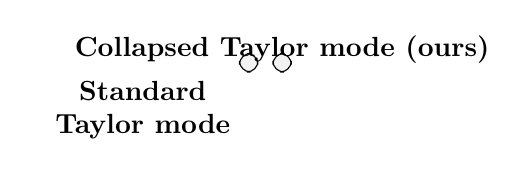
\begin{tikzpicture}
      \node (standard) [fill=black!5!white, draw=black, rounded corners]{\usebox{\taylorStandard}};
      \node [anchor=north east, align=center, inner sep=10pt] at (standard.north east) {\textbf{Standard} \\ \textbf{Taylor mode}};
      \node (collapsed) [fill=black!5!white, draw=black, rounded corners, anchor=north west, xshift=5pt] at (standard.north east) {\usebox{\taylorCollapsed}};
      \node [anchor=south, align=center, inner sep=3pt] at (collapsed.south) {\textbf{Collapsed Taylor mode (ours)}};
    \end{tikzpicture}
  }
  \caption{\textbf{Visual comparison of standard Taylor mode and our proposed collapsed Taylor mode.}}\label{fig:comparison-standard-vs-collapsed}
\end{figure*}

%%% Local Variables:
%%% mode: LaTeX
%%% TeX-master: "../main"
%%% End:
